We here consider the $Q_{k+1,k}\times Q_{k,k+1} \times Q_{k}^-$ element introduced 
by \textcite{huzh11} (2011).
The shape functions in 2D are in derived in Section~\ref{ss:qqq_elt}. 

The list of velocity degrees of freedom per element is as follows:
\[
\vec{\cal V} = (u_1,v_1,u_2,v_2,u_3,v_3,u_4,v_4,u_5,v_5,u_6,v_6)
\]
with the following internal numbering
\begin{verbatim}

u dofs      v dofs

4--6--3     4-----3
|     |     |     |
|     |     5     6
|     |     |     |
1--5--2     1-----2

\end{verbatim}
It is rather interesting to note that the location of the 'extra' 
nodes for u and v are opposite of those for the Fortin Q1+P0 element
(see stne 80).


We start with a simple $4\times 3$ element mesh.
Bubble $u$ dofs are represented in blue and bubble $v$ dofs are shown in red.


\begin{center}
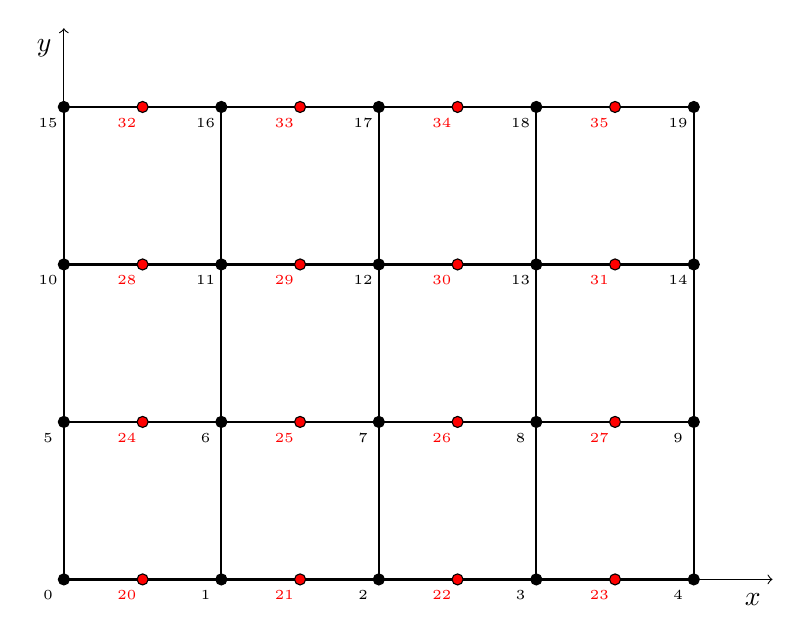
\begin{tikzpicture}
%\draw[fill=gray!23,gray!23](0,0) rectangle (10,8);
%\draw[step=0.5cm,gray,very thin] (0,0) grid (10,8); %background grid

\draw[thick] (1,1) -- (9,1) ;
\draw[thick] (1,3) -- (9,3) ;
\draw[thick] (1,5) -- (9,5) ;
\draw[thick] (1,7) -- (9,7) ;

\draw[thick] (1,1) -- (1,7) ;
\draw[thick] (3,1) -- (3,7) ;
\draw[thick] (5,1) -- (5,7) ;
\draw[thick] (7,1) -- (7,7) ;
\draw[thick] (9,1) -- (9,7) ;

\draw[black,fill=black] (1,1)   circle (2pt);
\draw[black,fill=black] (3,1)   circle (2pt);
\draw[black,fill=black] (5,1)   circle (2pt);
\draw[black,fill=black] (7,1)   circle (2pt);
\draw[black,fill=black] (9,1)   circle (2pt);

\draw[black,fill=black] (1,3)   circle (2pt);
\draw[black,fill=black] (3,3)   circle (2pt);
\draw[black,fill=black] (5,3)   circle (2pt);
\draw[black,fill=black] (7,3)   circle (2pt);
\draw[black,fill=black] (9,3)   circle (2pt);

\draw[black,fill=black] (1,5)   circle (2pt);
\draw[black,fill=black] (3,5)   circle (2pt);
\draw[black,fill=black] (5,5)   circle (2pt);
\draw[black,fill=black] (7,5)   circle (2pt);
\draw[black,fill=black] (9,5)   circle (2pt);

\draw[black,fill=black] (1,7)   circle (2pt);
\draw[black,fill=black] (3,7)   circle (2pt);
\draw[black,fill=black] (5,7)   circle (2pt);
\draw[black,fill=black] (7,7)   circle (2pt);
\draw[black,fill=black] (9,7)   circle (2pt);

\draw[black,fill=red] (2,1) circle (2pt); 
\draw[black,fill=red] (4,1) circle (2pt); 
\draw[black,fill=red] (6,1) circle (2pt); 
\draw[black,fill=red] (8,1) circle (2pt); 

\draw[black,fill=red] (2,3) circle (2pt); 
\draw[black,fill=red] (4,3) circle (2pt); 
\draw[black,fill=red] (6,3) circle (2pt); 
\draw[black,fill=red] (8,3) circle (2pt); 

\draw[black,fill=red] (2,5) circle (2pt); 
\draw[black,fill=red] (4,5) circle (2pt); 
\draw[black,fill=red] (6,5) circle (2pt); 
\draw[black,fill=red] (8,5) circle (2pt); 

\draw[black,fill=red] (2,7) circle (2pt); 
\draw[black,fill=red] (4,7) circle (2pt); 
\draw[black,fill=red] (6,7) circle (2pt); 
\draw[black,fill=red] (8,7) circle (2pt); 

\draw[thin,->] (9,1) -- (10,1); %x
\draw[thin,->] (1,7) -- (1,8); %y
\node[] at (9.75,0.75) {$x$};
\node[] at (0.75,7.75) {$y$};

\node[] at (0.8,0.8) {\tiny 0};
\node[] at (2.8,0.8) {\tiny 1};
\node[] at (4.8,0.8) {\tiny 2};
\node[] at (6.8,0.8) {\tiny 3};
\node[] at (8.8,0.8) {\tiny 4};
\node[] at (0.8,2.8) {\tiny 5};
\node[] at (2.8,2.8) {\tiny 6};
\node[] at (4.8,2.8) {\tiny 7};
\node[] at (6.8,2.8) {\tiny 8};
\node[] at (8.8,2.8) {\tiny 9};
\node[] at (0.8,4.8) {\tiny 10};
\node[] at (2.8,4.8) {\tiny 11};
\node[] at (4.8,4.8) {\tiny 12};
\node[] at (6.8,4.8) {\tiny 13};
\node[] at (8.8,4.8) {\tiny 14};
\node[] at (0.8,6.8) {\tiny 15};
\node[] at (2.8,6.8) {\tiny 16};
\node[] at (4.8,6.8) {\tiny 17};
\node[] at (6.8,6.8) {\tiny 18};
\node[] at (8.8,6.8) {\tiny 19};

\node[] at (1.8,0.8) {\tiny \color{red} 20};
\node[] at (3.8,0.8) {\tiny \color{red} 21};
\node[] at (5.8,0.8) {\tiny \color{red} 22};
\node[] at (7.8,0.8) {\tiny \color{red} 23};

\node[] at (1.8,2.8) {\tiny \color{red} 24};
\node[] at (3.8,2.8) {\tiny \color{red} 25};
\node[] at (5.8,2.8) {\tiny \color{red} 26};
\node[] at (7.8,2.8) {\tiny \color{red} 27};

\node[] at (1.8,4.8) {\tiny \color{red} 28};
\node[] at (3.8,4.8) {\tiny \color{red} 29};
\node[] at (5.8,4.8) {\tiny \color{red} 30};
\node[] at (7.8,4.8) {\tiny \color{red} 31};

\node[] at (1.8,6.8) {\tiny \color{red} 32};
\node[] at (3.8,6.8) {\tiny \color{red} 33};
\node[] at (5.8,6.8) {\tiny \color{red} 34};
\node[] at (7.8,6.8) {\tiny \color{red} 35};

\end{tikzpicture}
\end{center}








\input{python_codes/fieldstone_161/tikz_gridv}

For this mesh we have 

\begin{lstlisting}
nel=nelx*nely (=12) 
NP=nel (=12)
Nu=nnx*nny+nnx*nely (=20+16=36)
Nv=nnx*nny+nelx*nny (=20+15=35)
NV=nnx*nny+nnx*nely+nny*nelx (=20+16+15=51)
\end{lstlisting}

The total number of velocity dofs is 
\begin{lstlisting}
NfemV=ndofV*nnx*nny + nnx*nely + nny*nelx (=71)
\end{lstlisting}
while the total number of pressure dofs remains
\begin{lstlisting}
NfemP=NP*ndofP (=nel) 
\end{lstlisting}

What makes this element pair rather awkward to implement is the fact that 
there are two connectivity arrays {\tt iconu} and {\tt iconv}, both of size $mV\times nel$, where 
$mV=6$ is the number of nodes linked to an element for each velocity component. 
For each element, and depending on whether we are considering 
the polynomial approximation $u^h(x,y)$ or $v^h(x,y)$ in the element, there are the standard 4 $Q_1$ nodes and 2 additional 
dofs, so $mV=6$.
\begin{itemize}
\item content of {\tt iconu}
\begin{verbatim}
elt
0 | [ 0  1  6  5 35 39]
1 | [ 1  2  7  6 36 40]
2 | [ 2  3  8  7 37 41]
3 | [ 3  4  9  8 38 42]
4 | [ 5  6 11 10 39 43]
5 | [ 6  7 12 11 40 44]
6 | [ 7  8 13 12 41 45]
7 | [ 8  9 14 13 42 46]
8 | [10 11 16 15 43 47]
9 | [11 12 17 16 44 48]
10 | [12 13 18 17 45 49]
11 | [13 14 19 18 46 50]
\end{verbatim}
\item content of {\tt iconv}
\begin{verbatim}
elt
0 | [ 0  1  6  5 20 21]
1 | [ 1  2  7  6 21 22]
2 | [ 2  3  8  7 22 23]
3 | [ 3  4  9  8 23 24]
4 | [ 5  6 11 10 25 26]
5 | [ 6  7 12 11 26 27]
6 | [ 7  8 13 12 27 28]
7 | [ 8  9 14 13 28 29]
8 | [10 11 16 15 30 31]
9 | [11 12 17 16 31 32]
10 | [12 13 18 17 32 33]
11 | [13 14 19 18 33 34]
\end{verbatim}
\end{itemize}

Remark: given the weird placement of nodes for u and v, it makes sense not to 
use an isoparameteric mapping, and instead choose a Q2 mapping.

open question: quadrature for penalty term?
